\chapter{Results and conclusion}
\label{Sect:concl}
\vspace{-0.25em}



This study experimentally explores the process of charged double-pion electroproduction off protons bound in deuterium nuclei. The exploration became possible owing to the experiment of electron scattering off a deuterium target conducted in Hall B at Jefferson Lab with the CLAS detector~\cite{Mecking:2003zu}. The data collected in this experiment incorporates information on a broad range of physical phenomena that represent important blocks in our understanding of nuclear and particle interactions. Some of these phenomena are inherent in reactions off free protons as well, whereas others are unique for reactions off bound nucleons. 

In order to exploit to a higher degree opportunities offered by this deuteron target experiment, this study extends beyond the scope of observable extraction and represents an attempt at a broader and more detailed exploration of the features observed during the analysis. To facilitate understanding and interpretation of these features, the study~\cite{Fed_an_note:2017,Fed_paper_2018}, which analyzed the same exclusive reaction off free protons under the same experimental conditions, was used as a reference point. 

%\everypar{\looseness=-1}
As the main result of this study, the integral and single-differential cross sections~of the reaction $\gamma_{v}p(n) \rightarrow p' (n')\pi^{+}\pi^{-}$ in the kinematic region of the invariant mass $W$ from 1.3~GeV to 1.825~GeV and photon virtuality $Q^{2}$ from 0.4~GeV$^2$ to 1~GeV$^2$ have been obtained. The cross sections were extracted in the quasi-free regime, which means that the admixture of events with FSI was kinematically reduced to the achievable minimum.

\begin{figure}[htp]
\begin{center}
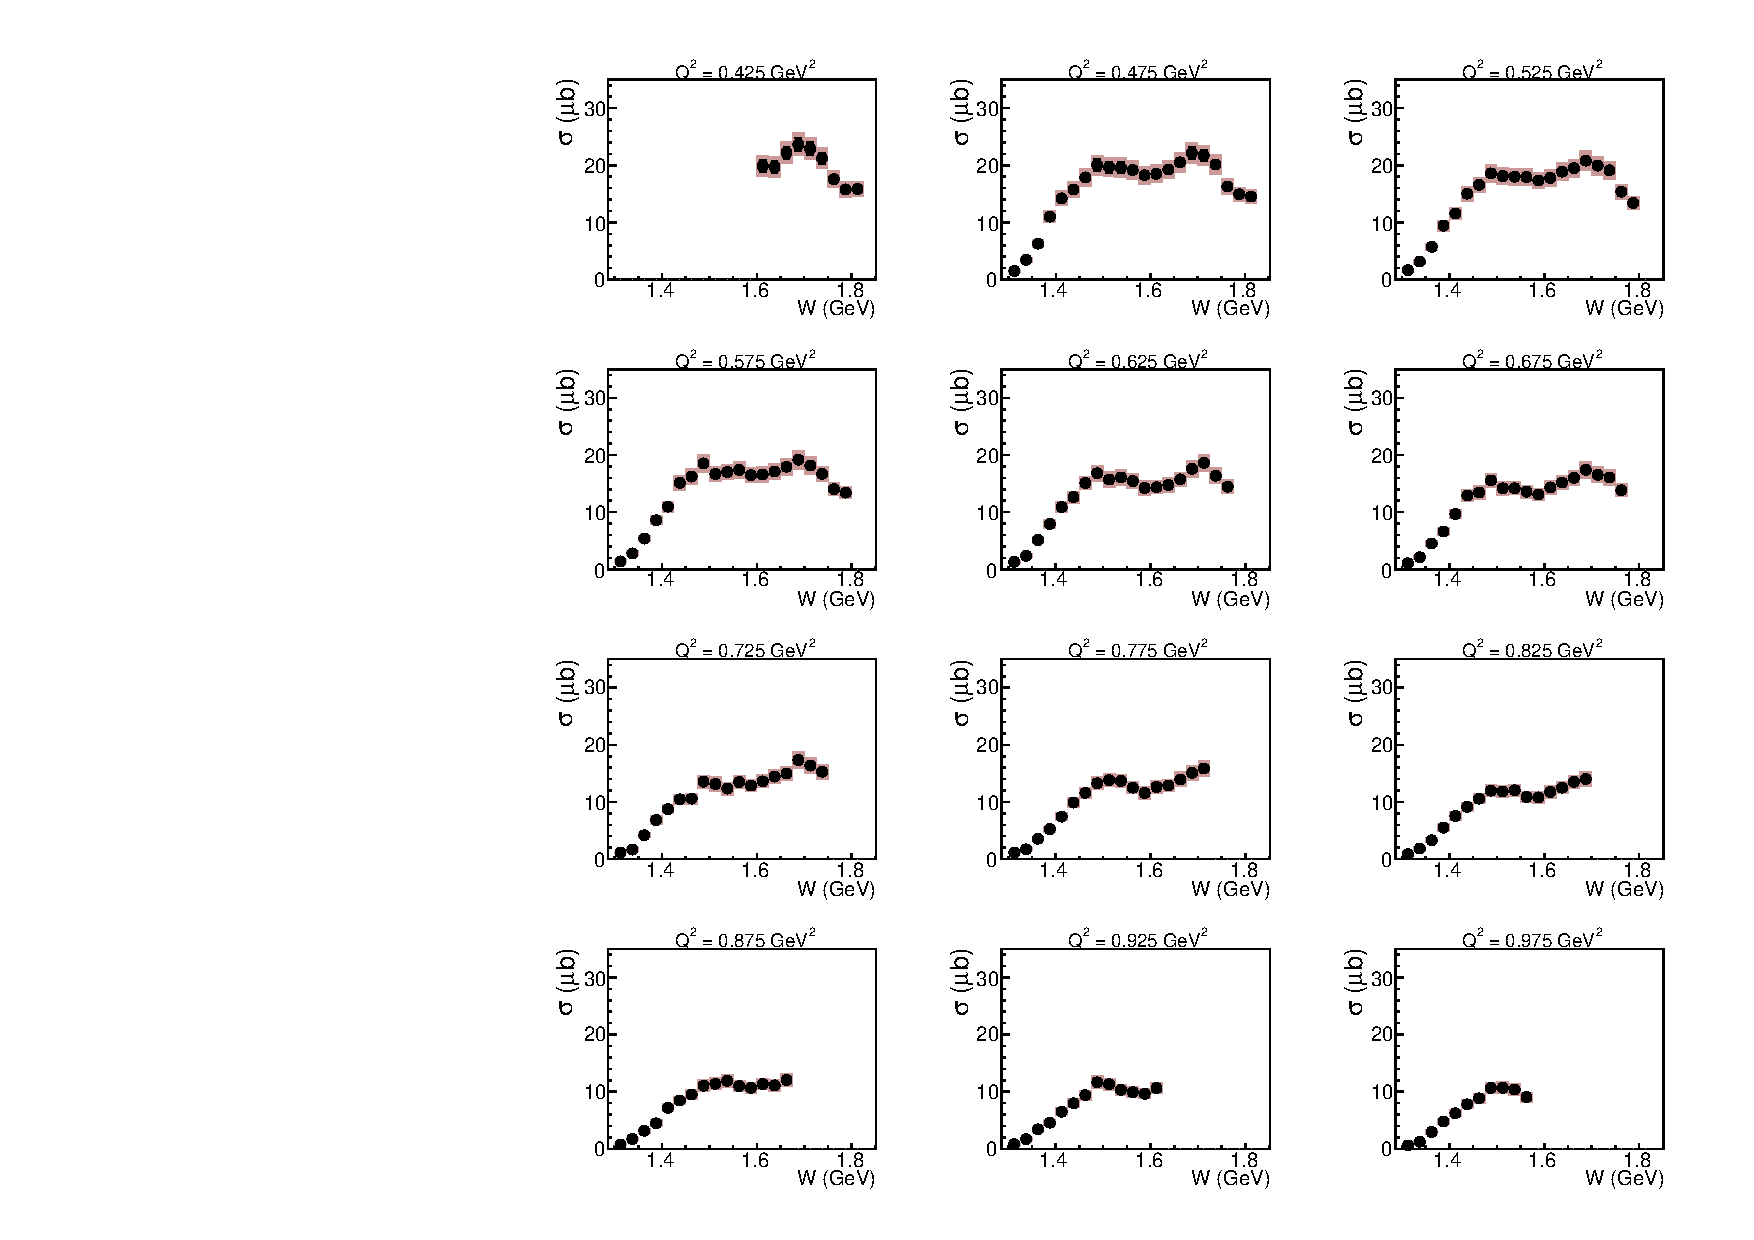
\includegraphics[width=\textwidth]{pictures/conclusion/wdep_20Jul2021.pdf}
\caption{\small $W$ dependences of the extracted integral cross sections in various bins in $Q^{2}$. The pink shadowed area for each point is the total cross section uncertainty, which is the uncertainty $\delta_{\text{stat,mod}}^{\text{tot}}$ (see Sect.~\ref{Sect:uncert_resume}) summed in quadrature with the total systematic uncertainty (see Sect.~\ref{Sect:sys_uncert}). The error bars that correspond to the $\delta_{\text{stat,mod}}^{\text{tot}}$ uncertainty only, are smaller than the symbol size.   } \label{fig:int_w_dep}
\end{center}
\end{figure}


\begin{figure}[htp]
\begin{center}
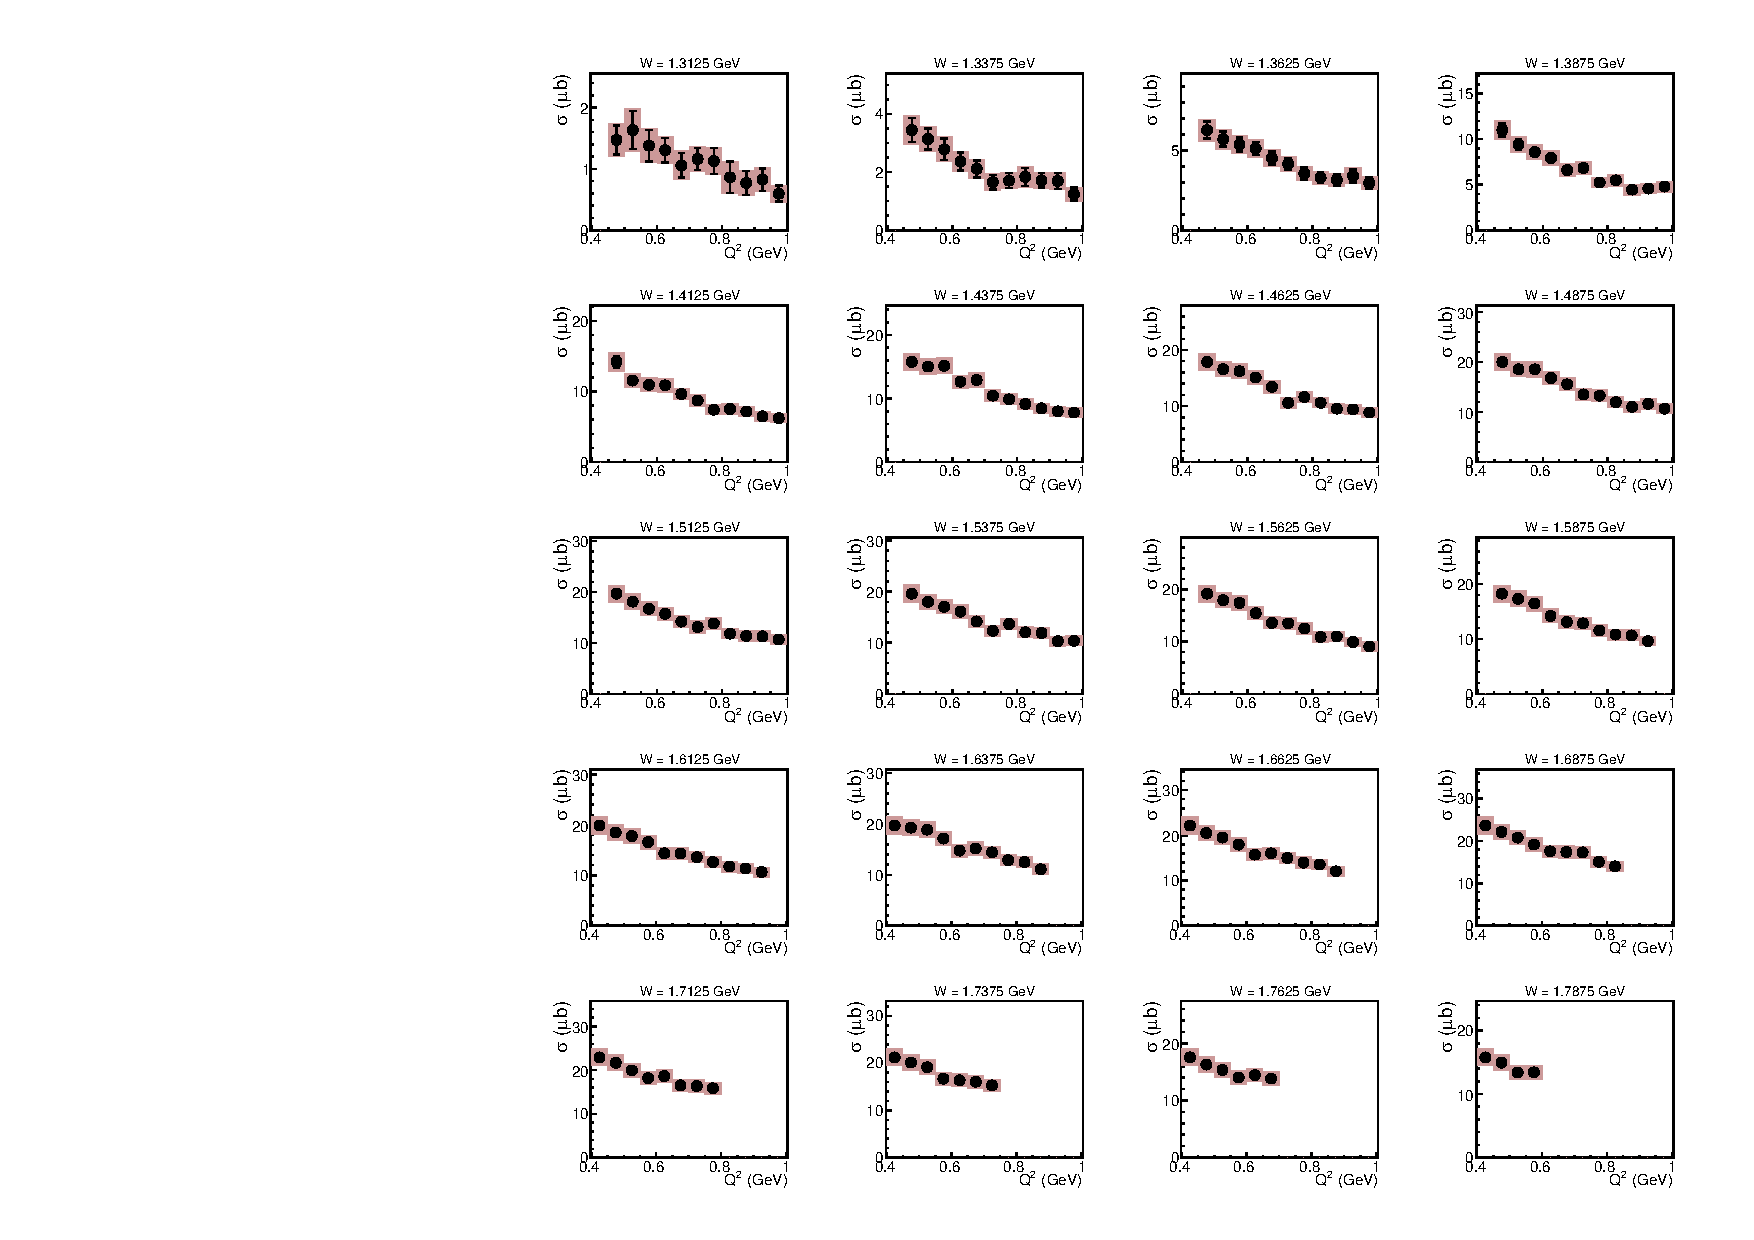
\includegraphics[width=\textwidth]{pictures/conclusion/q2dep_20Jul2021.pdf}
\caption{\small $Q^{2}$ dependences of the extracted integral cross sections in various bins in $W$. The pink shadowed area for each point is the total cross section uncertainty, which is the uncertainty $\delta_{\text{stat,mod}}^{\text{tot}}$ (see Sect.~\ref{Sect:uncert_resume}) summed in quadrature with the total systematic uncertainty (see Sect.~\ref{Sect:sys_uncert}). The error bars correspond to the $\delta_{\text{stat,mod}}^{\text{tot}}$ uncertainty only and for most of the points are smaller than the symbol size.  } \label{fig:int_q2_dep}
\end{center}
\end{figure}


\begin{figure}[htp]
\begin{center}
%\frame{}
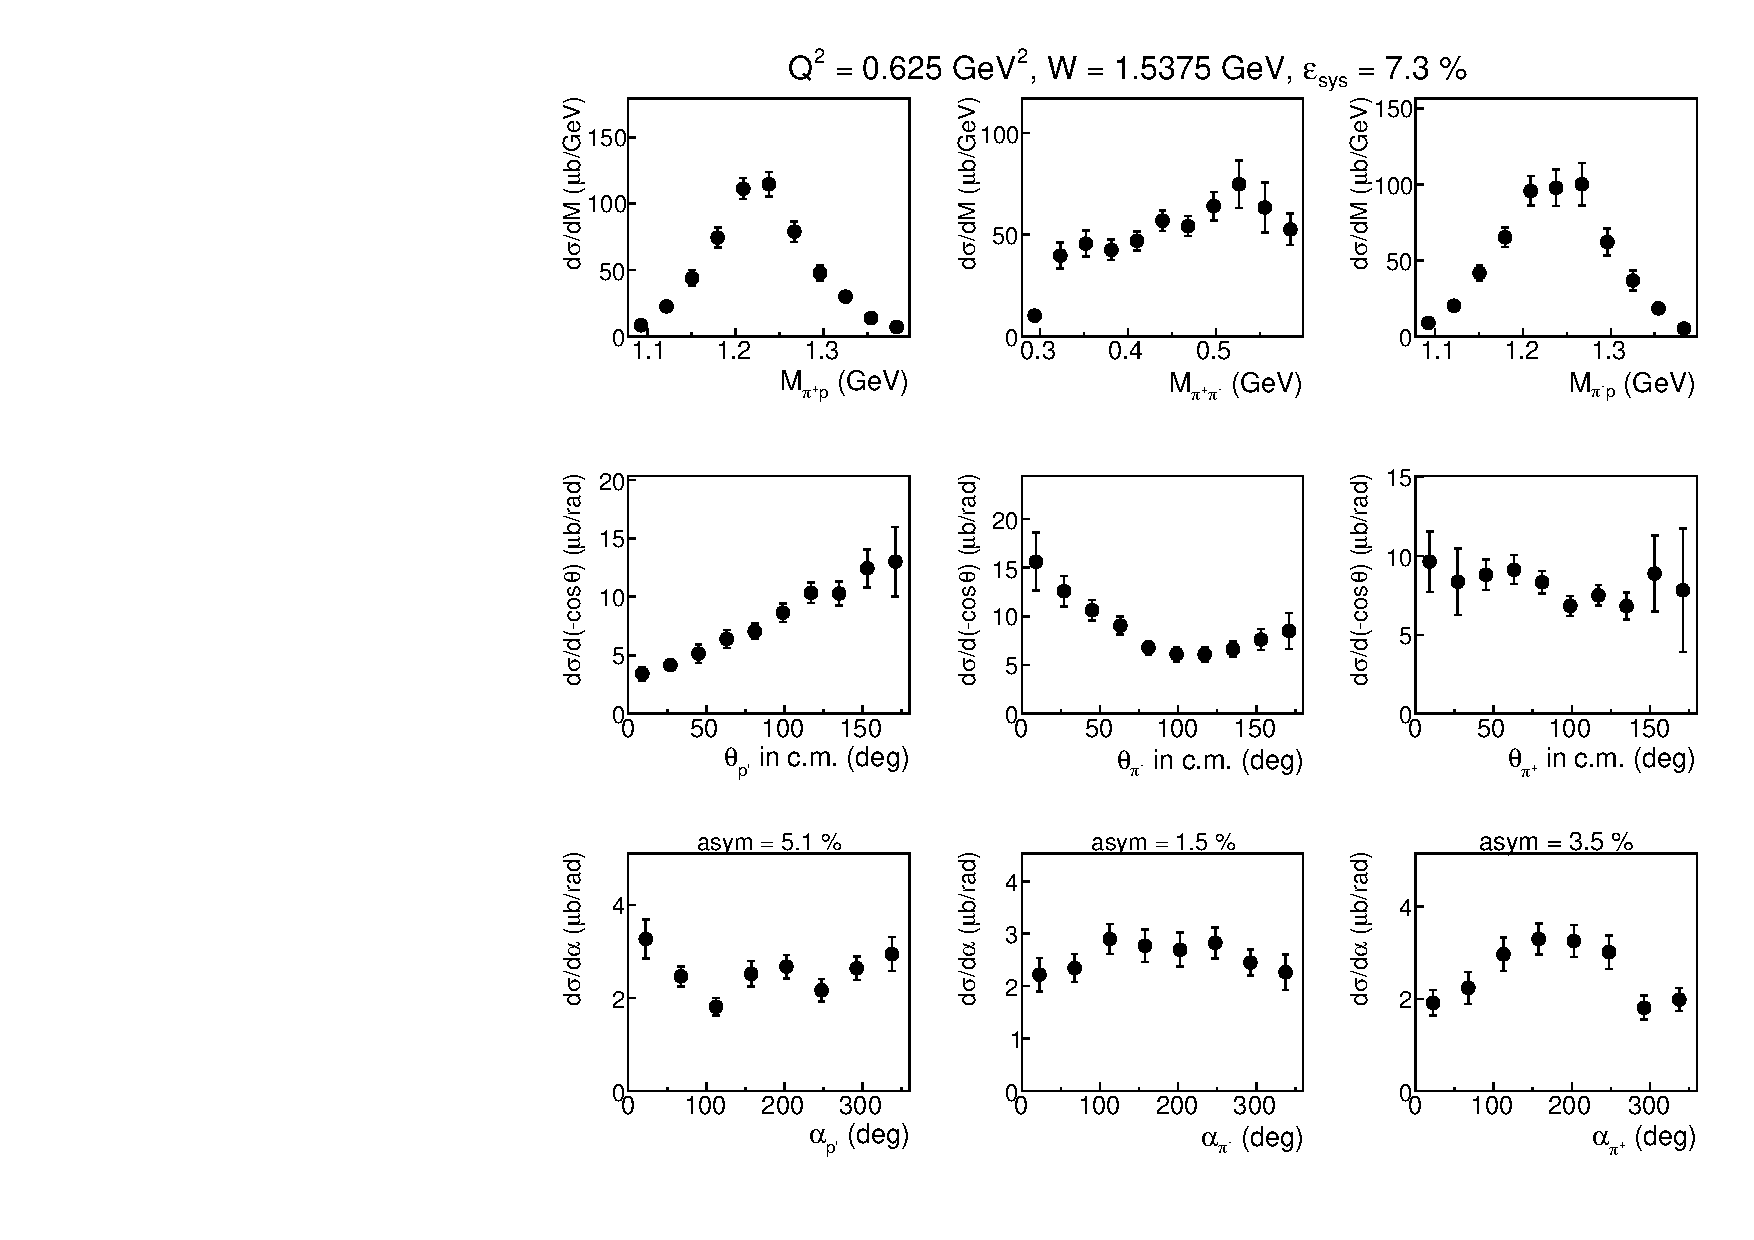
\includegraphics[width=\textwidth]{pictures/conclusion/w_15375.pdf}
\caption{\small Single-differential cross sections for $W= 1.5375$~GeV and $Q^{2}= 0.625$~GeV$^{2}$. The cross sections are shown with the uncertainty $\delta_{\text{stat,mod}}^{\text{tot}}$ represented by the error bars (see Sect.~\ref{Sect:uncert_resume}). The relative integral systematic uncertainty $\varepsilon_{\text{sys}}$ for this ($W$, $Q^{2}$) point is specified in the plot title. The definition of the average asymmetry factor specified above each $\alpha$ distribution, is given in App.~\ref{app_cr_sect}. }\label{fig:diff_plots}
\end{center}
\end{figure}



Figure~\ref{fig:int_w_dep} shows the $W$ dependences of the extracted integral cross sections in various bins in $Q^{2}$, while Figure~\ref{fig:int_q2_dep} shows their $Q^{2}$ dependences in various bins~in~$W$. The pink shadowed area for each point is the total cross section uncertainty, which is the uncertainty $\delta_{\text{stat,mod}}^{\text{tot}}$ (see Sect.~\ref{Sect:uncert_resume}) summed in quadrature with the total systematic uncertainty (see Sect.~\ref{Sect:sys_uncert}). The error bars correspond to the $\delta_{\text{stat,mod}}^{\text{tot}}$ uncertainty only and for most of the points are smaller than the symbol size.

For each integral cross section point, the set of nine single-differential cross sections has been obtained. As an example, Figure~\ref{fig:diff_plots} shows the single-differential cross sections for $W= 1.5375$~GeV and $Q^{2}= 0.625$~GeV$^{2}$. The cross sections are reported with the uncertainty $\delta_{\text{stat,mod}}^{\text{tot}}$ represented by the error bars. The value of the relative integral systematic uncertainty $\varepsilon_{\text{sys}}$ for this ($W$, $Q^{2}$) point is specified in the plot title. The full set of extracted single-differential cross sections is available in App.~\ref{app_cr_sect} accompanied by some explanatory remarks on the presentation format.


Note that FSI-background admixture left after the exclusivity cut in the $\pi^{-}$-missing topology (see Sect.~\ref{Sect:excl_cut_pim_miss}), being corrected only in an integral sense, may potentially impact the shape of extracted single-differential distributions (mostly angular). However, since this admixture is present only for events from the $\pi^{-}$-missing topology for $W>$~1.4625~GeV and stays there on the level of 3-7\%, its impact is not thought to be discernible against the total cross section uncertainty.

\everypar{\looseness=-1}
The cross section extraction analysis has undergone CLAS Collaboration Review by the Hadron Spectroscopy Working Group committee and been approved. 



The other outcome of this study consists in the performed kinematic examination of FSI between the reaction final hadrons and the spectator neutron for the process of $\pi^{+}\pi^{-}$ electroproduction off protons bound in deuterium nuclei. This examination counterbalances the main cross section extraction analysis, which was mainly focused on quasi-free events. 



The underlying idea of this examination stems from the fact that spectator nucleons are extrinsic to the original exclusive reaction, and therefore any interaction with them breaks the energy-momentum conservation imposed on the reaction particles. As a consequence, FSI with spectator nucleons introduce disturbances to the distributions of missing quantities, which can be examined along the reaction phase space. In this way, kinematic probing of this FSI type can be carried out.



In the performed examination, the increase in the relative amount of events with FSI in the regions of low momentum and large polar angles was observed for all final hadrons, to one extent or another. The dominance of proton-neutron interactions over the pion-neutron interactions was  also revealed. Besides this, in the regions with large FSI contribution kinematically available in this experiment, FSI were found to be dominated by the processes, in which non-relativistic protons lose their momentum.

In addition to that, pion-neutron FSI were shown to willingly evolve through the formation of resonances in the intermediate state, including those from the second resonance region. Due to multiple decay options available for the latter, such processes can then contribute to both elastic and inelastic FSI parts.



Further on, FSI manifestations were found to differ strongly depending on the reaction topology. This is because the probability to experience FSI differs for hadrons attributed to various topologies due to their non-identical geometrical acceptance.



It is also important that in reactions off bound nucleons, topologies with a missing hadron are revealed to suffer from miscounting of both quasi-free events and events with FSI as their separation is inaccurate. This inaccuracy originate from the fact that in such topologies the only quantity available for the channel identification and isolation of quasi free events is the missing mass of the unregistered particle, which does not reflect information on FSI of the missing hadron.% as its four-momentum is not included in the missing mass calculation. 



Meanwhile, the latter conclusion reveals one more potential uncertainty source for the extracted quasi-free cross sections. Specifically, for the $\pi^{-}$-topology, which is the main analysis topology, some of events with the $\pi^{-}$ FSI are falsely identified as quasi-free. The portion of such events is thought to be maximal near the reaction threshold and decline with growing $W$. Unfortunately, as true quasi-free events are kinematically identical to those that are falsely identified, this miscounting seems to be inevitable for any topology with a missing hadron in reactions off bound nucleons.


Another useful result of this analysis consists in exploring the effects of the initial proton motion. These effects turned out to be intertwined with many analysis aspects: they not only cause the smearing of some kinematic quantities, but also lead to the blurring of the boundaries of the $Q^{2}$ versus $W$ distributions, alter the common procedure of the Lab to CMS transformation, affect the population of the multi-dimensional cells, and more. On top of that, they affect the extracted quasi-free cross sections, causing the need to perform a special unfolding correction. These issues were subjected to a careful investigation, which to a high degree relied on the Monte Carlo simulation. The latter, meanwhile, was performed by means of the TWOPEG-D event generator~\cite{twopeg-d}, which was specially developed to deal with the effects of the initial proton motion in this study. 




Finally, in addition to the direct results summarized above, it is worthwhile to mention that this study initiated a set of related studies and developments. Among them are the development of the TWOPEG and TWOPEG-D event generators~\cite{twopeg,twopeg-d}, testing parameterizations of the deuteron quasi-elastic peak~\cite{note_QE_peak}, and exploration of peculiar features of missing mass distributions that includes an attempt of kinematic modeling of FSI effects~\cite{note_mm_distr}. Besides this, Ref.~\cite{Skorodumina:2015rea} and Ref.~\cite{Skorodumina:2016pnb} were also inspired by this analysis as well.%, which ucleon resonances in exclusive reactions of photo-and electroproduction of mesons





